
%(BEGIN_QUESTION)
% Copyright 2008, Tony R. Kuphaldt, released under the Creative Commons Attribution License (v 1.0)
% This means you may do almost anything with this work of mine, so long as you give me proper credit

Water treatment processes use chemicals called {\it flocculants} to force suspended solids to clump together and readily fall out of suspension.  Some flocculants such as polymers have the undesirable effect of lowering the water's pH value, which not only poses problems for further use of the water but also (ironically) minimizes flocculation efficiency.  In order to counter-act this decrease in pH, powdered lime may be added to the water in addition to flocculant to raise the pH level back to a more neutral value:

$$\includegraphics[width=15.5cm]{i03445x01.eps}$$

A pH transmitter measures the pH level of the water exiting the mixing tank, on its way to the clarifier where the floc will settle to the bottom over time and cleaner water is collected at the outer rim.

\vskip 10pt

If someone happens to change the setpoint on the flocculant flow controller, the flow of powdered lime into the mixing tank will not change until the pH controller (AIC) sees a change in pH, which by then may be too late to make a swift correction.  The result will be a ``bump'' in pH over time that may take a while to correct. 

Modify this control system to include feedforward, so that any change in flocculant flow rate will {\it immediately} alter the flow rate of lime, in order to help stabilize pH and thereby improve water treatment quality.

\vskip 20pt \vbox{\hrule \hbox{\strut \vrule{} {\bf Suggestions for Socratic discussion} \vrule} \hrule}

\begin{itemize}
\item{} Perhaps the most common mistake made in this problem is to place the feedforward summing function block at the PV input to a controller, when it should actually be located at the output of a controller instead.  Explain how we may determine the correct location for the summing block in the control scheme of this process, and/or explain why the other location is wrong.
\item{} For those who have previously studied chemistry, explain what {\it pH} is and why it is important.
\item{} Why is a {\it mixing tank} important to have in a system like this where pH is being continuously controlled?
\end{itemize}

\underbar{file i03445}
%(END_QUESTION)





%(BEGIN_ANSWER)

$$\includegraphics[width=15.5cm]{i03445x02.eps}$$
 
%(END_ANSWER)





%(BEGIN_NOTES)


%INDEX% Control, strategies: feedforward
%INDEX% Process: municipal water flocculation

%(END_NOTES)


